\section{Einleitung}
\begin{figure}[h!]
  \centering
    \reflectbox{%
      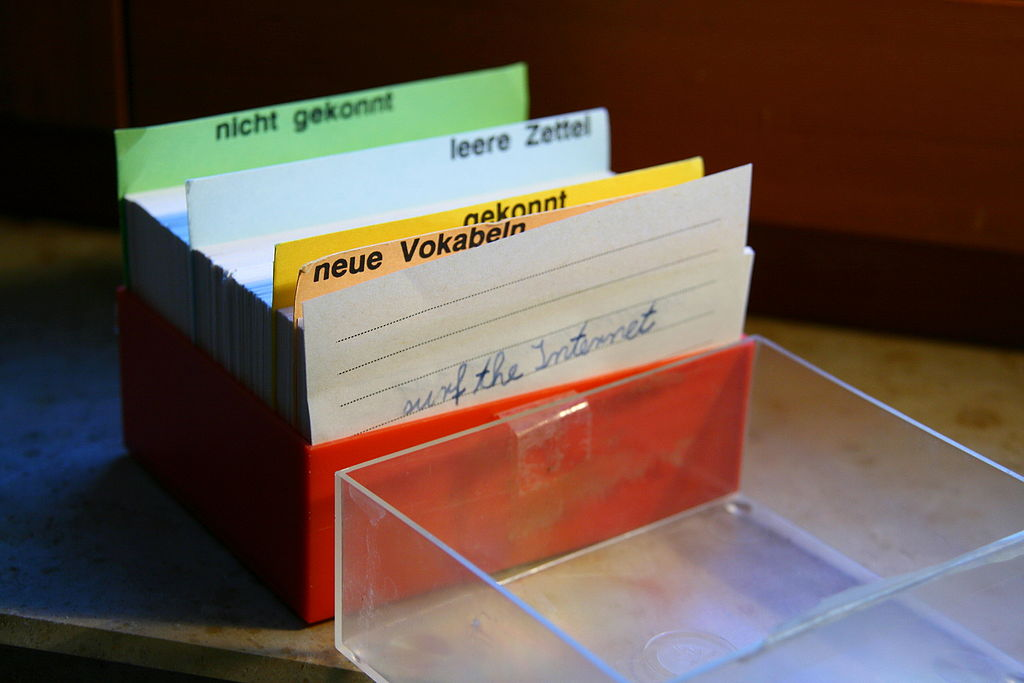
\includegraphics[scale=1]{images/1024px-Lernkartei_Vokabelbox.jpg} }
  \caption[Lernkartei Vokabelbox]{Lernkartei Vokabelbox\footnotemark}
\end{figure}
\footnotetext{By Stefan-Xp (Own work) [\href{http://www.gnu.org/copyleft/fdl.html}{GFDL} or \href{http://creativecommons.org/licenses/by-sa/3.0/)}{CC-BY-SA-3.0}], via Wikimedia Commons}

\noindent Unser Projekt überträgt die Idee von physischen Lernkarten auf eine digitale Webseite. Lernkarten bieten sich an um Vokabeln für Fremdsprachen und Definitionen für andere Themen auswendig zu lernen. Die Bedienung der Webseite soll einfach sein, damit sich der Benutzer auf das Lernen konzentrieren kann. 